\documentclass[11pt]{article}
\usepackage[margin=1in]{geometry}
\usepackage{amsmath,amssymb,graphicx,booktabs,listings,xcolor,hyperref,enumitem}
\usepackage{tcolorbox}
\hypersetup{colorlinks=true,linkcolor=blue!60!black,urlcolor=blue!60!black}
\definecolor{codebg}{RGB}{247,247,245}
\lstset{language=Python,basicstyle=\ttfamily\small,backgroundcolor=\color{codebg},frame=single,framerule=0pt,
  keywordstyle=\color{blue!60!black},commentstyle=\color{gray},stringstyle=\color{green!40!black},
  showstringspaces=false,breaklines=true,columns=fullflexible,xleftmargin=4pt,xrightmargin=4pt}
\newtcolorbox{exercise}[1]{colback=blue!3,colframe=blue!50!black,title={Exercise #1},fonttitle=\bfseries,left=4pt,right=4pt}
\newtcolorbox{checkbox}{colback=green!4,colframe=green!40!black,title={What to compare against},fonttitle=\bfseries,left=4pt,right=4pt}
\newtcolorbox{vocab}{colback=orange!4,colframe=orange!60!black,title={Vocabulary},fonttitle=\bfseries,left=4pt,right=4pt}
\newcommand{\eps}{\varepsilon}
\newcommand{\code}[1]{\texttt{#1}}
\newcommand{\F}{\mathbb{F}}
\title{Monte Carlo beyond the exact engine:\\ thresholds of the large codes, correlated outputs, and biased noise}
\author{prime\_msd project notes for Aanha, part II}
\date{31 October 2026}

\begin{document}
\maketitle
\tableofcontents

\section{Where we are}

Part~I asked you to validate the exact performance engine (\code{qmsd/performance.py})
with the channel-level sampler \code{qmsd.mc\_distill.simulate}, on codes small enough
that the exact curve exists. This part assumes that pipeline works for you: you can
build $G_0$ and $H_1$ for any catalog record, draw errors, post-select on the
syndrome, and count logical failures with error bars.

Three things happened in the project since Part~I was written, and each opens a
question that only sampling can answer.

\begin{enumerate}[nosep]
\item \textbf{The large codes have no threshold.} The paper's headline codes,
  $[[1756,260,7]]_7$ and $[[1746,270,7]]_7$ (overhead exponent $\gamma<1$), and the
  $p\ge 17$ ladder ($[[296,65,6]]_{19}$ up to $[[766,195,{\ge}6]]_{31}$), have
  stabiliser spaces of dimension 15--66. The exact engine enumerates $p^{\dim A}$
  words; $7^{66}$ is not a number anyone enumerates. So the performance table shows a
  dash in the threshold column for every code the paper is actually about.
\item \textbf{We now have rigorous bounds, and they are loose.} Section~\ref{sec:bg}
  explains them. The rigorous threshold of $[[1756,260,7]]_7$ is $0.34\%$; the true
  value is certainly higher, and nobody knows by how much. A sampled curve between
  $0.2\%$ and $1\%$ answers that directly.
\item \textbf{Every cost number assumes independent inputs.} A multi-round protocol
  is costed by composing single-round curves, which treats the inputs of round two as
  independent. They are not: an accepted weight-7 error of $[[1756,260,7]]_7$ flips
  6--12 of its 260 outputs at once (Figure~\ref{fig:corr}, left). Nobody has measured
  what that does to the next round for a high-rate qudit code.
\end{enumerate}

Add a fourth, smaller question a referee will ask: the engine assumes the noise is
\emph{twirled} (every nonzero $Z$-power equally likely). What if it is not?

\subsection{Your three tasks}

\begin{description}[nosep]
\item[A. Thresholds of the large codes by sampling] (Section~\ref{sec:A}). Measure
  $\eps_{\rm out}(\eps)$ for the six codes of Table~\ref{tab:large} between $0.2\%$
  and $1\%$, locate the crossing $\eps_{\rm out}=\eps$ by bisection, and put the result
  next to the rigorous bound. Deliverable: Figure~\ref{fig:window} with your points,
  and one threshold per code with an error bar. \emph{This is the one to do first: it
  produces numbers the paper lacks and it reuses your Part~I harness unchanged.}
\item[B. The correlation test] (Section~\ref{sec:B}). Measure how failures of the
  outputs of one block are correlated, then run a two-round protocol with the
  round-two inputs taken from a single block versus shuffled across blocks.
  Deliverable: the within-block statistics table and the two-routing comparison.
\item[C. Biased noise] (Section~\ref{sec:C}). Replace the uniform distribution over
  $Z$-powers by a biased one and measure how the output error moves. Deliverable: one
  bias sweep per code for three codes.
\end{description}

Every number quoted below was produced by
\code{docs/aanha\_mc\_guide2/make\_figures.py}; rerun it to regenerate them. Keep
the house rules: \code{PYTHONPATH=.} from the repo root, \code{ulimit -v 4000000},
\code{OMP\_NUM\_THREADS=1}, results in small JSON files, plots last.

\section{Background}
\label{sec:bg}

\subsection{Bounded curves: what is proved about a large code}

For a small code the engine computes the exact per-output error
$\eps_{\rm out}(\eps)$. For a large code we know three things: the distance $d$
(certified), the number $A_d$ of weight-$d$ error vectors that pass the syndrome check
and how many outputs each one flips (the \emph{census}), and nothing about heavier
accepted errors except that they exist. From these, \code{qmsd/rigorous\_curve.py}
builds two curves that bracket the truth:
\begin{align*}
f_{\rm lo}(\eps) &= \frac{L_d\,(\eps/(p-1))^d (1-\eps)^{n-d}}{P_{\rm acc}^{\rm hi}(\eps)},\qquad
f_{\rm hi}(\eps) = \frac{L_d\,(\eps/(p-1))^d (1-\eps)^{n-d} + \sum_{w>d}\binom{n}{w} p^{\,w-d+1} (\eps/(p-1))^w (1-\eps)^{n-w}}{(1-\eps)^{n}} .
\end{align*}
Here $L_d$ is the per-output average number of weight-$d$ failing vectors (from the
census), the denominator of $f_{\rm hi}$ is the acceptance of the zero error alone,
and the sum counts \emph{every} heavier accepted error as a failure with the
Singleton bound $N_w\le\binom{n}{w}p^{w-d+1}$ on how many there can be (inside any
$w$ coordinates the code has distance $\ge d$, so at most $p^{w-d+1}$ words live
there). The \emph{surrogate} used in \code{PERFORMANCE.md} keeps only the first
term with $P_{\rm acc}\approx(1-\eps)^n$: $\eps_{\rm out}\approx c_\eps\,\eps^d$ with
$c_\eps = L_d/(p-1)^d$.

\begin{vocab}
\textbf{Bounded curve}: a pair $(f_{\rm lo}, f_{\rm hi})$ with
$f_{\rm lo}\le\eps_{\rm out}\le f_{\rm hi}$ proved for every $\eps$.
\textbf{Rigorous threshold}: the largest $\eps$ with $f_{\rm hi}(\eps)<\eps$; below it
one round provably improves the state. \textbf{Surrogate}: the leading term
$c_\eps\eps^d$ alone, exact as $\eps\to0$, unproved elsewhere.
\textbf{Singleton tail}: the $\sum_{w>d}$ term; it over-counts heavier accepted errors by
roughly $p^{\dim A}$, which is why $f_{\rm hi}$ is far above the truth.
\end{vocab}

Figure~\ref{fig:window} shows the two curves for $[[1756,260,7]]_7$. At
$\eps=10^{-6}$ they differ by sixteen orders of magnitude; the rigorous threshold is
$0.34\%$ while the surrogate, having no higher-order terms, crosses the
diagonal only at an absurd 85\%. The true threshold is somewhere between, and the
only way to find it is to sample. The shaded band is where sampling is affordable
(next subsection).

\begin{figure}[t]\centering
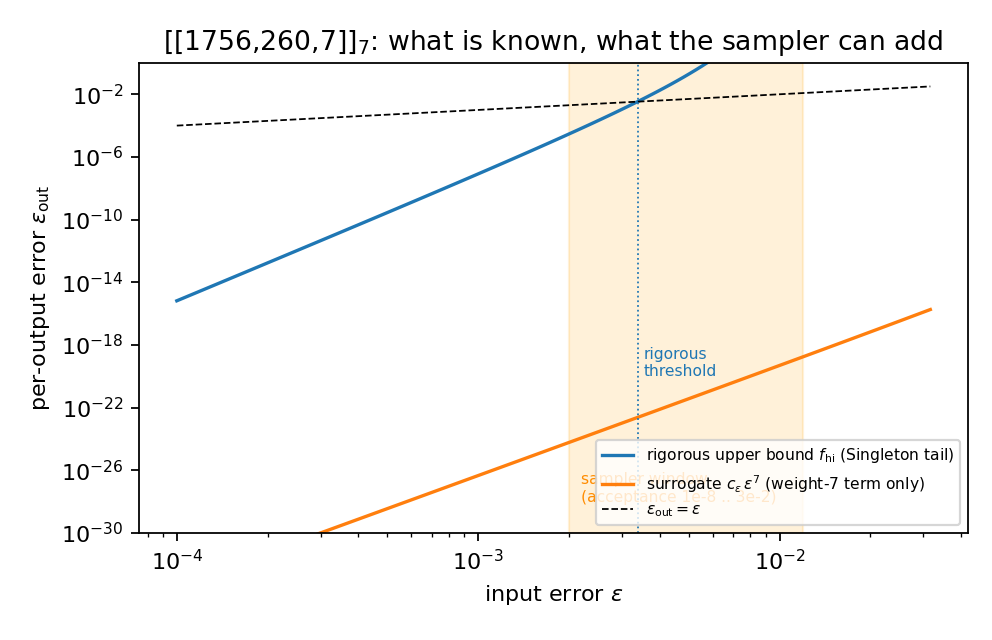
\includegraphics[width=0.78\textwidth]{fig_rigorous_window.png}
\caption{$[[1756,260,7]]_7$: the rigorous upper bound, the surrogate, and the
diagonal. Your points go in the orange band.}
\label{fig:window}
\end{figure}

A fact worth knowing before you start, because it tells you what to expect: with the
\emph{proved} curves the distillation cost of $[[1756,260,7]]_7$ keeps its full
$4.1\times$ saving over the standard $p=7$ library at $10^{-2}\to10^{-30}$, while the
$d=5,6$ codes $[[2093,308,5]]_7$ and $[[1746,270,6]]_7$ keep only $1.3\times$ of their
surrogate $4.1$--$4.3\times$. The proof rewards distance; the surrogate rewards rate.
Your sampled curves live at much higher $\eps$ than either protocol uses, but they
decide which picture is closer to reality near threshold, which is where a real
device would run the first round.

\subsection{Postselection statistics}

Sampling a distillation round means drawing $N$ error vectors, keeping the
$N_{\rm acc}\approx N P_{\rm acc}$ that pass the syndrome check, and counting
failures among them. Two numbers control the cost and the precision.

\begin{itemize}[nosep]
\item \textbf{Acceptance.} $P_{\rm acc}(\eps) = (1-\eps)^n$ to within a percent for
  every large code (Part~I measured this). At $n=1756$ this is $17\%$ at
  $\eps=10^{-3}$, $0.5\%$ at $3\times10^{-3}$ and $2\times10^{-8}$ at $10^{-2}$
  (Figure~\ref{fig:acc}). Above about $7\times10^{-3}$ you cannot collect accepted
  blocks at all for the $p=7$ codes; for the shorter $p\ge19$ codes the window
  extends to a few percent.
\item \textbf{Failures.} The relative error of a failure rate estimated from
  $N_{\rm fail}$ observed failures is $1/\sqrt{N_{\rm fail}}$, independent of
  everything else. Ten failures give $30\%$, a hundred give $10\%$. Near threshold
  $\eps_{\rm out}\sim\eps$, so a few hundred accepted blocks already contain
  failures; far below threshold you will see none, and the right statement is then an
  upper bound ($\eps_{\rm out} < (1-1/p)\,3/N_{\rm acc}$ at 95\%, because a failing block
  usually hits most of its outputs).
\end{itemize}

\begin{figure}[t]\centering
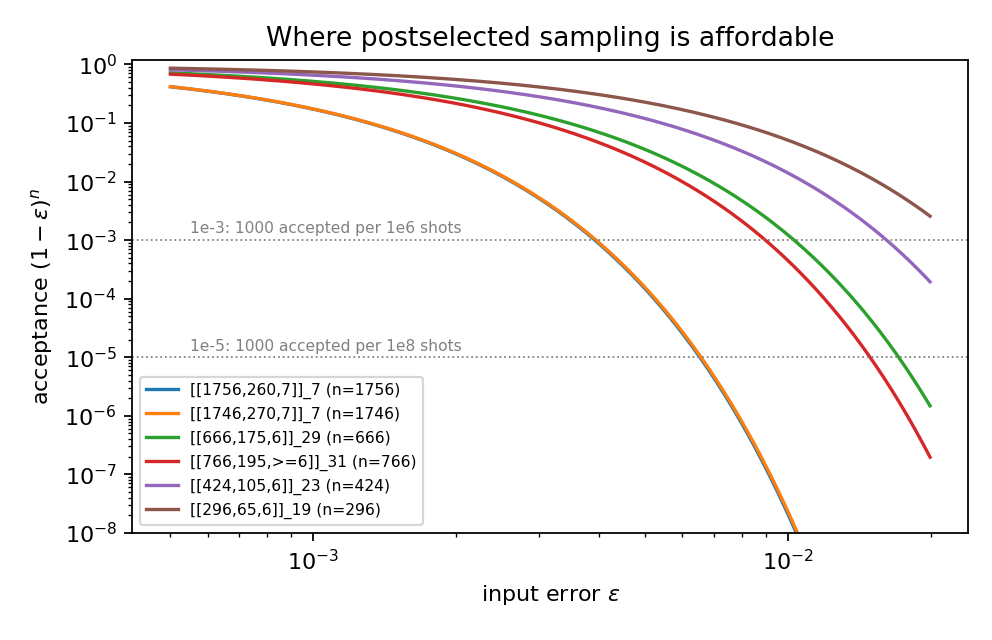
\includegraphics[width=0.78\textwidth]{fig_acceptance.png}
\caption{Acceptance of the six large codes. A run of $10^6$ shots yields $1000$
accepted blocks where a curve crosses the upper dotted line.}
\label{fig:acc}
\end{figure}

\begin{vocab}
\textbf{Shots}: error vectors drawn. \textbf{Accepted blocks}: shots passing the
syndrome check. \textbf{Per-output error}: failures counted over all $k N_{\rm acc}$
outputs; \textbf{block error}: accepted blocks with at least one failed output. The
paper quotes the per-output number; the block number is what you see first because it
is larger. \textbf{Poisson error bar}: $\sqrt{N_{\rm fail}}$ on a count, hence
$1/\sqrt{N_{\rm fail}}$ relative.
\end{vocab}

\subsection{Bisection with a noisy function}

The threshold is the root of $g(\eps) = \eps_{\rm out}(\eps)/\eps - 1$. Ordinary
bisection halves an interval by the sign of $g$ at its midpoint; with a sampled $g$
the sign is only reliable when $|g|$ exceeds its error bar. The practical rule: at
each midpoint, draw shots until either the sign is three standard deviations clear or
you reach a shot budget; if the budget runs out, stop and report the interval. Near
the root $g$ is small and the error bars dominate, so expect to resolve the threshold
to $10$--$20\%$, not to three digits. That is enough: the paper needs ``$0.9\%$'' next
to the rigorous ``$0.34\%$'', not $0.913\%$.

\subsection{What the engine assumes between rounds}

A protocol $C_1\to C_2$ is costed as $\eps\mapsto f_1(\eps)\mapsto f_2(f_1(\eps))$,
with cost $\prod n_i/(k_i P_{{\rm acc},i})$. The second step takes $f_2$ at the
\emph{marginal} per-output error of round one, which is correct only if the $n_2$
inputs of a round-two block fail independently. The outputs of one round-one block
do not: a single accepted error vector $e$ fails every output $i$ with
$h_i\cdot e\ne0$ simultaneously, and for high-rate codes the logical rows $h_i$ are
dense, so one accepted error typically flips a sizeable fraction of the outputs.
Round two then sees either no bad input or many at once, and its distance-$d_2$
protection is defeated by the ``many'' case far more often than the independent
calculation says. Whether this matters in practice depends on how the outputs are
routed: if the $n_2$ inputs of a round-two block come from $n_2$ \emph{different}
round-one blocks, independence holds exactly. Task~B measures both.

\begin{vocab}
\textbf{Joint failure}: two outputs of the same block failing in the same shot.
\textbf{Pair ratio}: $P(i\text{ and }j\text{ fail})/[P(i\text{ fails})P(j\text{ fails})]$;
$1$ means independent. \textbf{Routing}: which round-one blocks feed a round-two
block. \textbf{Same-block routing}: all inputs from one block (worst case);
\textbf{shuffled routing}: each input from a different block (the engine's
assumption).
\end{vocab}

\subsection{Biased noise and one symmetry}

The engine's noise is $(1-\eps)\,\rho + \frac{\eps}{p-1}\sum_{j\ne0} Z^j\rho Z^{-j}$:
with probability $\eps$ a nontrivial power of $Z$, all powers equally likely. A biased
channel keeps the total $\eps$ but weights the powers: we use
$w_{j^*} = b + (1-b)/(p-1)$ for one favoured power $j^*$ and $w_j=(1-b)/(p-1)$ for
the others, so $b=0$ is the twirled model and $b=1$ is a single power. One symmetry
saves you work: multiplying an error vector by a nonzero scalar $a$ maps accepted
errors to accepted errors ($\ker G_0$ is linear) and failures to failures
($a\,h_i\cdot e\ne0$ iff $h_i\cdot e\ne0$), so \emph{which} power is favoured never
matters, only the shape of the distribution. Exercise~C1 checks this.

\section{Task A: thresholds of the large codes}
\label{sec:A}

\subsection{The codes}

\begin{table}[h]\centering\footnotesize
\begin{tabular}{llrrrrr}
\toprule
code & catalog id & $P_{\rm acc}(0.2\%)$ & $P_{\rm acc}(0.3\%)$ & $P_{\rm acc}(0.5\%)$ & $P_{\rm acc}(1\%)$ & shots/1000 acc.\ (0.3\%) \\
\midrule
\relax$[[1756,260,7]]_{7}$ & \code{imported-p7-n1756-k260-9d263f2240e4} & $3.0\times10^{-2}$ & $5.1\times10^{-3}$ & $1.5\times10^{-4}$ & $2.2\times10^{-8}$ & $2.0\times10^{5}$ \\
\relax$[[1746,270,7]]_{7}$ & \code{imported-p7-n1746-k270-c93a88f0735a} & $3.0\times10^{-2}$ & $5.3\times10^{-3}$ & $1.6\times10^{-4}$ & $2.4\times10^{-8}$ & $1.9\times10^{5}$ \\
\relax$[[666,175,6]]_{29}$ & \code{imported-p29-n666-k175-4f8ad426d19b} & $2.6\times10^{-1}$ & $1.4\times10^{-1}$ & $3.5\times10^{-2}$ & $1.2\times10^{-3}$ & $7.4\times10^{3}$ \\
\relax$[[766,195,{\ge}6]]_{31}$ & \code{imported-p31-n766-k195-8cc6fbf9e4da} & $2.2\times10^{-1}$ & $1.0\times10^{-1}$ & $2.2\times10^{-2}$ & $4.5\times10^{-4}$ & $1.0\times10^{4}$ \\
\relax$[[424,105,6]]_{23}$ & \code{imported-p23-n424-k105-9d5204d5ccf4} & $4.3\times10^{-1}$ & $2.8\times10^{-1}$ & $1.2\times10^{-1}$ & $1.4\times10^{-2}$ & $3.6\times10^{3}$ \\
\relax$[[296,65,6]]_{19}$ & \code{imported-p19-n296-k65-211e1fbb4b1a} & $5.5\times10^{-1}$ & $4.1\times10^{-1}$ & $2.3\times10^{-1}$ & $5.1\times10^{-2}$ & $2.4\times10^{3}$ \\
\bottomrule
\end{tabular}
\caption{The large codes, their catalog ids (\code{record\_matrices} rebuilds $G_0$,
$H_1$ from the id as in Part~I, Appendix~A) and the acceptance that sets your shot
budget. $[[766,195,{\ge}6]]_{31}$ has $d\in\{6,7\}$; your sampled curve cannot tell
which, but its threshold does not need to.}
\label{tab:large}
\end{table}

The two $p=7$ codes are the paper's headline and the hardest to sample (acceptance
falls fastest because $n$ is largest). The $p\ge19$ codes are cheap and should be
done first as practice. The matrices are integer arrays of shape
$(\dim A, n)$ and $(k, n)$; for the weighted $p=7$ codes \code{record\_matrices}
takes a few seconds because it rebuilds the charge support.

\subsection{The recipe}

\begin{enumerate}[nosep]
\item For each code, run \code{simulate} at $\eps\in\{0.2, 0.3, 0.5, 0.7\}\%$ (and
  $1\%$, $2\%$ for $p\ge19$) with a shot budget chosen from Table~\ref{tab:large} so
  that each point has at least 1000 accepted blocks; $10^6$--$10^7$ shots per point.
  The sampler processes $2\times10^5$ shots per batch; at $n=1756$ a batch is
  $1756\times2\times10^5$ integers, about 2.8\,GB at 64 bits, so lower \code{batch}
  to $5\times10^4$ for the $p=7$ codes or you will hit the memory cap.
\item Record $P_{\rm acc}$, $\eps_{\rm out}^{\rm avg}$, $\eps_{\rm out}^{\rm block}$
  and the raw counts (shots, accepted, failures). The counts are what let you combine
  runs later.
\item Plot $\eps_{\rm out}^{\rm avg}$ against $\eps$ on log--log axes with the
  diagonal, $f_{\rm hi}$ and the surrogate (Figure~\ref{fig:window};
  \code{qmsd.rigorous\_curve.from\_census} gives $f_{\rm hi}$ for the three $p=7$
  codes with censuses; for the others use the Singleton tail with $L_d$ unknown, i.e.\
  plot only the tail).
\item Bisect for the crossing as in Section~\ref{sec:bg}.
\end{enumerate}

\begin{exercise}{A1: acceptance only}
Run $[[296,65,6]]_{19}$ at $\eps=1\%$ with $10^5$ shots and compare $P_{\rm acc}$
with $(1-\eps)^{296}$.
\end{exercise}
\begin{checkbox}
$(0.99)^{296} = 0.0511$; you should land within $0.002$ of it. If you are far off,
your $G_0$ is wrong (most likely a transposed matrix or a missing \code{\% p}).
\end{checkbox}

The second exercise is the first real measurement. Below threshold most accepted
blocks are clean, so you will see few failures; that is the point, and the number of
failures is what sets your error bar.

\begin{exercise}{A2: one point on a large code}
Run $[[424,105,6]]_{23}$ at $\eps=1\%$ with $2\times10^6$ shots. Report $P_{\rm acc}$,
the number of failed outputs, $\eps_{\rm out}^{\rm avg}$ with its error bar, and
$\eps_{\rm out}^{\rm avg}/\eps$.
\end{exercise}
\begin{checkbox}
About $2.8\times10^4$ accepted blocks. Whether you see failures depends on where the
true threshold lies, which is exactly what we do not know; if the ratio
$\eps_{\rm out}/\eps$ is clearly below~1 you are below threshold. Either way, write
down the 95\% upper bound $(1-1/p)\,3/N_{\rm acc}$ if you saw no failure. (Corrected 4 November: this
guide first said $3/(k N_{\rm acc})$, which assumes a failing block hits one output. A generic kernel word hits a
fraction $1-1/p$ of them; on $[[1746,270,7]]_7$ the census gives about $0.7$.)
\end{checkbox}

Now the bisection. Do it on a cheap code first so that you can afford to be wasteful
with shots and see the method work.

\begin{exercise}{A3: bisection on a cheap code}
Find the threshold of $[[296,65,6]]_{19}$ between $0.5\%$ and $5\%$: evaluate
$g(\eps)=\eps_{\rm out}/\eps-1$ at the geometric midpoint, draw shots until its sign
is $3\sigma$ clear (cap $10^7$ shots), halve, repeat until the interval is within
$15\%$ of itself.
\end{exercise}
\begin{checkbox}
Expect three to five midpoints. Report the final interval, the shots spent, and the
sampled $\eps_{\rm out}$ at both ends. Sanity: at the lower end
$\eps_{\rm out}/\eps$ should be well below 1; near the crossing a large fraction of
accepted blocks have failed outputs.
\end{checkbox}

\begin{exercise}{A4: the six codes}
Repeat A3 for all six codes of Table~\ref{tab:large}. For the two $p=7$ codes start
the interval at $[0.2\%, 0.7\%]$ and use \code{batch=50\_000}; if the crossing is
above $0.7\%$ you will not be able to resolve it (acceptance $<10^{-5}$), and the
honest result is ``threshold $>0.7\%$, $\eps_{\rm out}(0.7\%) = \ldots$''.
\end{exercise}
\begin{checkbox}
One number per code with an interval, plus the point measurements, in a JSON. Put
the rigorous thresholds next to them: $0.34\%$ for $[[1756,260,7]]_7$; for the
$p\ge19$ codes compute them with \code{RigorousBoundCurve(name,p,n,k,d,L\_d=0,A\_d=0)}
(no census: the weight-$d$ term is dropped, which only makes the bound \emph{less}
pessimistic, so state it as ``tail-only'').
\end{checkbox}

The last exercise is the comparison the paper will print.

\begin{exercise}{A5: the figure}
Produce Figure~\ref{fig:window} for $[[1756,260,7]]_7$ and $[[1746,270,7]]_7$ with
your points and error bars, and a one-line table: code, rigorous threshold, sampled
threshold, ratio.
\end{exercise}
\begin{checkbox}
A measured crossing must exceed the rigorous threshold (if not, one of the two is wrong
and it is almost certainly a convention: check that your $\eps$ is the probability of
a nontrivial $Z$-power, not the repository's $\delta = p\eps/(p-1)$). A lower bound from zero
failures can lie below the rigorous threshold, and then it adds nothing to the proof; say so. Only a
sampled value above the rigorous one measures how loose the proof is.
\end{checkbox}

\section{Task B: are the outputs of one block independent?}
\label{sec:B}

\subsection{Within-block statistics}

The sampler returns totals; this task needs the per-shot failure matrix
$F\in\{0,1\}^{N_{\rm acc}\times k}$ (Appendix~\ref{app:code} has a 12-line sampler that
returns it). From $F$: the marginals $m_i = \bar F_{\cdot i}$, the joint
$P_{ij} = \overline{F_{\cdot i}F_{\cdot j}}$, the pair ratio $P_{ij}/(m_i m_j)$, and
the number of failed outputs per failing block.

Two reference runs (Table~\ref{tab:corr}) show how far from independent the outputs
are. For $[[99,22,3]]_{11}$ at $\eps=3\%$ a failing block has on average
$7.1$ of its 22 outputs wrong; independence would give a second failure in
$0.05\%$ of failing blocks, the sample gives $100\%$. The pair ratio is in the
thousands. The qutrit $[[200,43,3]]_3$ is worse: $26$ of 43 outputs fail together.
This is the regime where routing matters.

\begin{table}[h]\centering\small
\begin{tabular}{lrrrrrr}
\toprule
code & $\eps$ & accepted & $\eps_{\rm out}^{\rm avg}$ & $\eps_{\rm out}^{\rm block}$ & failures per failing block & pair ratio (mean) \\
\midrule
$[[99,22,3]]_{11}$ & 0.01 & 739461 & $3.1\times10^{-7}$ & $1.4\times10^{-6}$ & 5.0 & (one failing block) \\
$[[99,22,3]]_{11}$ & 0.03 & 98265 & $2.3\times10^{-5}$ & $7.1\times10^{-5}$ & 7.1 & 30087 \\
$[[200,43,3]]_{3}$ & 0.005 & 732894 & $2.2\times10^{-5}$ & $3.8\times10^{-5}$ & 25.1 & 27929 \\
$[[200,43,3]]_{3}$ & 0.01 & 267974 & $2.0\times10^{-4}$ & $3.4\times10^{-4}$ & 25.9 & 3042 \\
\bottomrule
\end{tabular}
\caption{Reference within-block statistics ($2\times10^6$ shots each, seed 3,
\code{make\_figures.py}). ``Failures per failing block'' is the mean number of wrong
outputs in blocks with at least one; independence would make it $1+(k-1)\eps_{\rm out}\approx1$.}
\label{tab:corr}
\end{table}

\begin{figure}[t]\centering
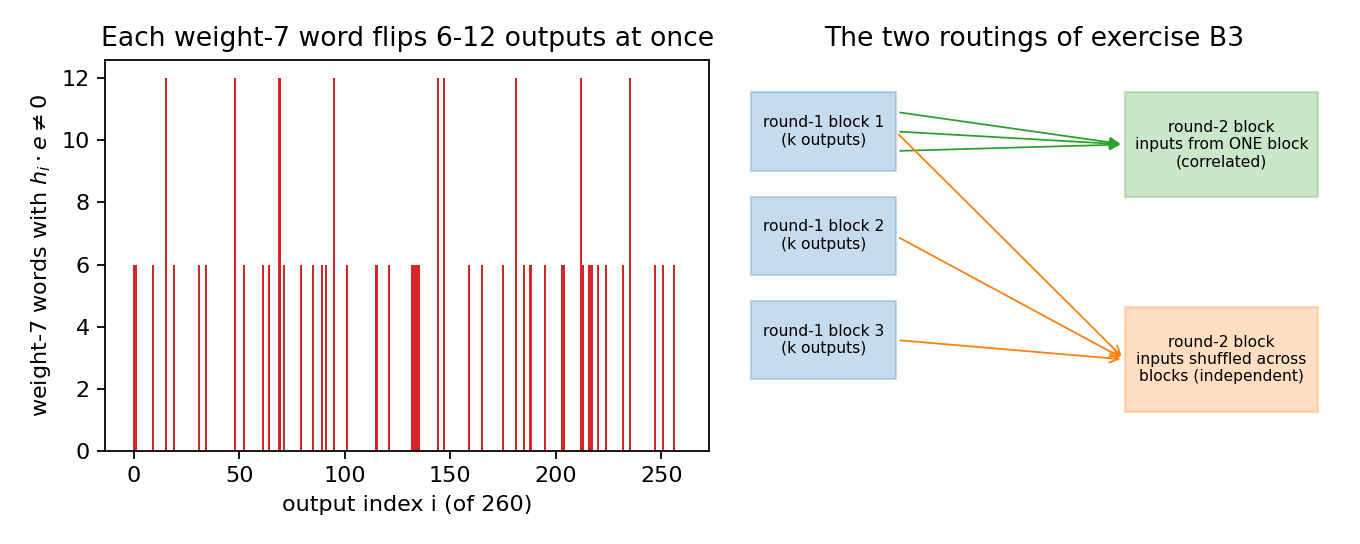
\includegraphics[width=0.98\textwidth]{fig_correlation.png}
\caption{Left: how the 24 weight-7 words of $[[1756,260,7]]_7$ are distributed over
its outputs (census): 47 of 260 outputs are touched, some by 12 words. Right: the
two routings of Exercise~B3.}
\label{fig:corr}
\end{figure}

\begin{exercise}{B1: reproduce the statistics}
Write the per-shot sampler (or copy Appendix~\ref{app:code}), run $[[99,22,3]]_{11}$
at $\eps=3\%$ with $2\times10^6$ shots, and compute the four columns of
Table~\ref{tab:corr}. Check that the marginal mean equals \code{simulate}'s
$\eps_{\rm out}^{\rm avg}$ for the same seed.
\end{exercise}
\begin{checkbox}
Table~\ref{tab:corr}, row 2, to within the Poisson error of 14 failing blocks
($\pm30\%$ on the block error; the per-failing-block mean is much more stable).
\end{checkbox}

\begin{exercise}{B2: why}
For $[[99,22,3]]_{11}$ list the accepted weight-3 vectors (enumerate all
$\binom{99}{3}10^3$ or use \code{structured\_ad.mitm\_streamed(G0, 3, 11)}), and for
each count the outputs $i$ with $h_i\cdot e\ne0$. Compare the histogram with the
``failures per failing block'' you measured.
\end{exercise}
\begin{checkbox}
At $\eps=1\%$ almost every failing block fails through a single weight-3 vector, so the
measured mean (5.0 in the reference run) is just the number of outputs that vector
touches. At $3\%$ heavier vectors contribute and the mean rises to 7.1.
\end{checkbox}

\subsection{The two-round experiment}

Choose a round-two code $C_2$ with $n_2 \le k_1$, so that a round-two block can be
filled from a single round-one block. Feed round two in two ways
(Figure~\ref{fig:corr}, right): \emph{same-block}, the first $n_2$ outputs of one
accepted round-one block; \emph{shuffled}, $n_2$ outputs drawn from $n_2$ different
accepted blocks. The input errors are the actual residual $Z$-powers
($h_i\cdot e \bmod p$ for output $i$, which is what the magic state carries into the
next round), not a resampled Bernoulli. Round two applies its own syndrome check and
failure count. Measure $\eps_{\rm out,2}$ both ways and compare with the engine's
composition $f_2(\eps_{\rm out,1})$.

A concrete pair: $C_1 = [[99,22,3]]_{11}$ at $\eps=3\%$ and $C_2 = [[10,1,4]]_{11}$
(Reed--Solomon, $n_2=10\le22$; catalog id from \code{SMALL\_CODES.md}), or the same
with $C_1=[[200,43,3]]_3$ and $C_2 = [[19,1,3]]_3$. Round one's per-output error is
$\sim 2\times10^{-5}$ at $3\%$, so with independent inputs round two almost never
fails and you need many round-one blocks; with same-block routing the failures
cluster and round two fails whenever a cluster lands inside its block. Budget: $10^7$
round-one shots, which is a few minutes.

\begin{exercise}{B3: two routings}
Implement the experiment for one of the two pairs. Report, for each routing: the
number of round-two blocks, accepted, failed; $\eps_{\rm out,2}$; and the engine's
prediction $f_2(\eps_{\rm out,1})$ from the exact curve of $C_2$
(\code{profile\_exact}, Part~I Appendix~B).
\end{exercise}
\begin{checkbox}
Shuffled routing should agree with the engine within error bars (this is the
engine's assumption made true by construction). Same-block routing should be
\emph{worse by orders of magnitude}: with 7 of 22 outputs failing together, a
10-input block from the same round-one block contains $\ge d_2=4$ bad inputs in a
large fraction of the failing cases, so round two inherits round one's block error
rate instead of suppressing it. Quote the ratio.
\end{checkbox}

\begin{exercise}{B4: what a protocol should do}
Write one paragraph for the paper: when does same-block routing arise in practice
(a factory that consumes a block's outputs together), what the measured penalty is,
and why shuffling across $n_2$ blocks removes it at no cost in states. Include the
one number a reader needs: the round-two failure ratio from B3.
\end{exercise}

\section{Task C: biased noise}
\label{sec:C}

The sampler changes in one line: draw the nonzero value with weights instead of
uniformly (\code{rng.choice(np.arange(1,p), p=weights)} in place of
\code{rng.integers(1,p)}; Appendix~\ref{app:code}). For the smallest codes the effect
can be computed exactly by enumerating all $p^n$ error vectors
(\code{exact\_biased} in Appendix~\ref{app:code}, $7^7 = 823{,}543$ vectors for
$[[7,1,3]]_7$), which gives you reference numbers with no statistical error.

\begin{figure}[t]\centering
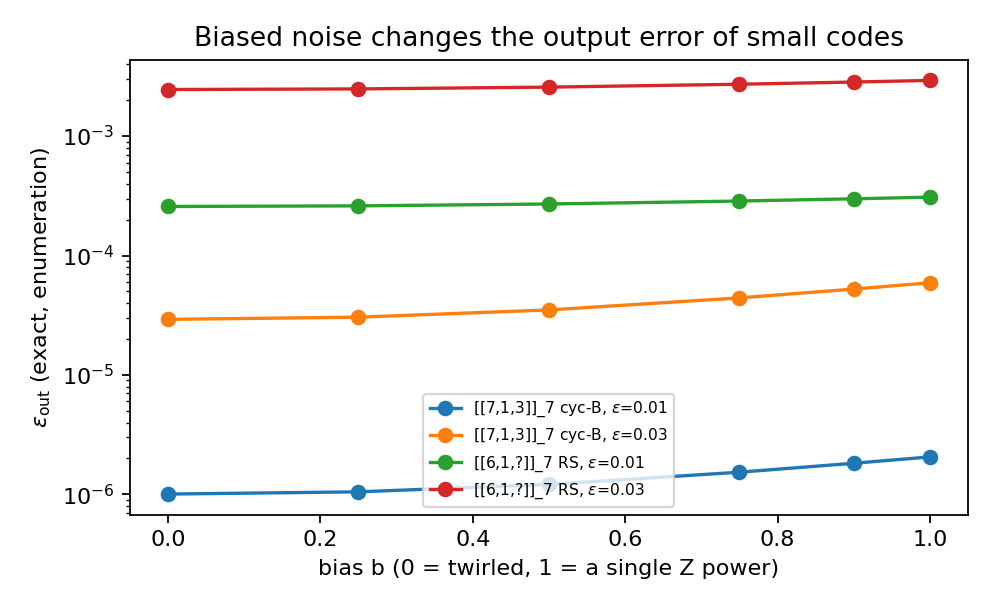
\includegraphics[width=0.7\textwidth]{fig_biased.png}
\caption{Exact output error of the two smallest $p=7$ codes against the bias $b$.}
\label{fig:bias}
\end{figure}

Figure~\ref{fig:bias} shows the effect on $[[7,1,3]]_7$ and the Reed--Solomon
$[[6,1,{?}]]_7$: at $\eps=1\%$ full bias raises $\eps_{\rm out}$ of $[[7,1,3]]_7$ from
$1.0\times10^{-6}$ to $2.1\times10^{-6}$, a factor~2, and of the RS code by only 20\%.
The reason is the coefficient pattern of the lightest accepted errors: a weight-3
accepted vector of $[[7,1,3]]_7$ has a specific ratio of its three coefficients, and a
biased channel that produces equal powers is more or less likely to hit that ratio
than a uniform one. Acceptance barely moves ($<10^{-4}$ relative).

\begin{exercise}{C1: the symmetry}
Compute (exactly) $\eps_{\rm out}$ of $[[7,1,3]]_7$ at $\eps=1\%$, $b=0.9$, favouring
each of the six powers $j^*=1,\dots,6$ in turn.
\end{exercise}
\begin{checkbox}
Six identical numbers, $1.8\times10^{-6}$. If they differ, your failure test is not
scale-invariant (it must test $h_i\cdot e\ne0$, not $h_i\cdot e = 1$).
\end{checkbox}

\begin{exercise}{C2: reproduce the figure by sampling}
Sample $[[7,1,3]]_7$ at $\eps=3\%$ for $b\in\{0, 0.5, 1\}$ with $4\times10^6$ shots and
overlay the points on Figure~\ref{fig:bias}.
\end{exercise}
\begin{checkbox}
$\eps_{\rm out} = 2.9\times10^{-5}$, $3.5\times10^{-5}$, $5.9\times10^{-5}$
with $P_{\rm acc} = 0.8080$; about 150 failures per point, so $\pm8\%$.
\end{checkbox}

\begin{exercise}{C3: a search code}
Repeat C2 for $[[111,10,6]]_{11}$ (id \code{imported-p11-n111-k10-51e7da182d60}) at
$\eps=5\%$ and for $[[296,65,6]]_{19}$ at $\eps=2\%$, $b\in\{0,0.5,0.9,1\}$. Report the
ratio $\eps_{\rm out}(b=1)/\eps_{\rm out}(b=0)$.
\end{exercise}
\begin{checkbox}
No reference number exists; this is new. Expect factors between $0.3$ and $3$. A
ratio far outside that range is interesting and should be checked by enumerating the
lightest accepted vectors (as in B2) and looking at their coefficient patterns: a
code whose weight-$d$ words all have equal coefficients is the most bias-sensitive.
\end{checkbox}

\section{Deliverables}

\begin{enumerate}[nosep]
\item \textbf{Task A}: a JSON with every point (code, $\eps$, shots, accepted,
  failures, $\eps_{\rm out}$, error) and the six thresholds with intervals;
  Figure~\ref{fig:window} for the two $p=7$ codes with your points; the one-line
  table of rigorous versus sampled thresholds. This goes straight into
  \code{PERFORMANCE.md} and the paper.
\item \textbf{Task B}: Table~\ref{tab:corr} reproduced and extended to one more
  code; the two-routing comparison with the engine's prediction; the paragraph of B4.
\item \textbf{Task C}: C1's six numbers, C2's overlay, C3's two ratios.
\end{enumerate}

Order: A1--A3 (one afternoon), A4--A5 (a day of machine time, little of yours), then
B, then C. If A4's bisection on the $p=7$ codes stalls because the crossing is above
$0.7\%$, do not burn a week on it: report the bound and move on; the shorter codes
carry the same message.

\appendix
\section{Code}\label{app:code}

Per-shot failure matrix (returns \code{F} of shape (accepted, $k$)); with
\code{weights} it samples the biased channel:
\begin{lstlisting}
import numpy as np
def sample_failures(G0, H1, p, eps, shots, seed=0, batch=100_000, weights=None):
    G0 = np.asarray(G0) % p; H1 = np.asarray(H1) % p; n = G0.shape[1]
    rng = np.random.default_rng(seed); out = []; vals = np.arange(1, p)
    for s in range(0, shots, batch):
        b = min(batch, shots - s)
        v = rng.choice(vals, size=(b, n), p=weights) if weights is not None else rng.integers(1, p, size=(b, n))
        j = np.where(rng.random((b, n)) < eps, v, 0)
        ok = ~np.any((j @ G0.T) % p, axis=1)
        out.append(((j[ok] @ H1.T) % p) != 0)
    return np.concatenate(out)
\end{lstlisting}
For Task~B keep the residual values as well: replace the last line of the loop by
\code{out.append((j[ok] @ H1.T) \% p)}; a nonzero entry is both ``failed'' and the
$Z$-power the next round receives.

Bias weights and the exact enumeration for tiny codes:
\begin{lstlisting}
import itertools
def bias_weights(p, b):
    base = (1 - b) / (p - 1); return [b + base] + [base] * (p - 2)   # favours j* = 1
def exact_biased(G0, H1, p, eps, weights):
    G0 = np.asarray(G0) % p; H1 = np.asarray(H1) % p; n = G0.shape[1]
    allv = np.array(list(itertools.product(range(p), repeat=n)), dtype=np.int64)
    acc = allv[~np.any((allv @ G0.T) % p, axis=1)]
    w = np.array([1 - eps] + [eps * x for x in weights]); pr = np.prod(w[acc], axis=1)
    fail = ((acc @ H1.T) % p != 0).any(axis=1)
    return float(pr.sum()), float(pr[fail].sum() / pr.sum())       # P_acc, eps_out (block = avg for k = 1)
\end{lstlisting}
The standard $p=7$ codes: \code{from qmsd.cyclic import construction\_B;
G0, H1 = construction\_B(7, 8, \{1, 4, 7\})} is $[[7,1,3]]_7$; the Reed--Solomon
$[[6,1,{?}]]_7$ is RM$(1,1)$ over $\F_7$ punctured at one point, built exactly as the
$[[8,1,2]]_3$ snippet of Part~I with \code{p, m = 7, 1}. The rigorous curve:
\code{from qmsd.rigorous\_curve import from\_census; c =
from\_census("runs/weighted/p7\_m4\_sphere\_1756\_260\_7\_census.json"); c.f\_hi(eps),
c.threshold\_eps}.

\section{Files}
\begin{itemize}[nosep]
\item \code{qmsd/rigorous\_curve.py}: the bounded curves; \code{PERFORMANCE.md}
  (section ``Rigorous bounds behind the surrogate'') explains the proved-versus-surrogate
  reversal.
\item \code{runs/weighted/*census.json}: the weight-$d$ censuses ($A_d$, per-output
  counts) of the three large $p=7$ codes.
\item \code{docs/aanha\_mc\_guide2/make\_figures.py}: every figure and number here;
  \code{numbers.json} has them in machine-readable form.
\item \code{docs/aanha\_mc\_guide/}: Part~I (the sampler walk-through, the exact
  engine, building $G_0$ and $H_1$).
\end{itemize}

\end{document}
